\section{Producing intermediate surface pretilt}
\label{cha:pretilt}
As has been shown in Chapter \ref{cha:splay_uniform}, the bulk director profile under flow can be greatly affected by the presence of a relatively small amount of pretilt of the director at the boundary layer. For example, it has been seen that the starting director profile (made different via the rubbing direction and hence direction of the pretilt) can lead to dramatically different director profiles when subjected to a pressure gradient. A seemingly natural progression from this finding is then to ask, \textit{can we increase this effect by using much larger initial pretilt angles?} 

As will be seen in Chapter \ref{cha:diode}, a large amount of pretilt can indeed be used to dramatically alter the effect of director orientation when subjected to a pressure gradient. However, we shall also see in this chapter that the methods and techniques used to obtain such high pretilt angles of the director are of great scientific interest and appear to work with varying levels of success.

Experimentally, two techniques are characterised for their ability to produce intermediate pretilt angles for both of the liquid crystals 5CB and ZLI-2293 (Merck). Briefly, these two methods involve, 1) the `over-baking' (baking at temperatures much higher than the manufacturer's guidelines) and rubbing of polymer alignment layers conventionally used for vertical alignment, and 2) the doubling up of alignment layers by depositing a planar aligning polyimide on top of a vertical aligning polyimide. Results from these experiments suggest that the surface upon which the aligning layer is deposited plays a crucial role in the production of these intermediate pretilt angles, and also that the surface energy of the subsequent aligning layer gives little or no indication of the magnitude of pretilt that will be produced. Some of the results presented in this chapter concerning the second, double polyimide layer, recipe appear to be in contradiction with some existing results from the relevant literature.

\subsection{Introduction}
\label{sec:pretilt_introduction}
Liquid crystal displays have now been in use worldwide for nearly 30 years. Yet, which came as both a surprise and curiosity, the mechanism responsible for liquid crystal alignment on mechanically buffed polymer films is still poorly understood \citep{Kumar2005}. Since this method of mechanical alignment plays a crucial role in the production of the majority of these displays, it is interesting to try to understand the physical reason that lies behind the observation that a nematic liquid crystal will tend to align itself on a rubbed polymer film with the director parallel to the direction of rubbing.

Purely qualitatively, a simple consideration of the relevant length scales seems to suggest that a conventional nematic liquid crystal molecule shouldn't `see' the grooves and scratches created by a cotton or velvet cloth that has buffed the surface of a thin polymer layer. The analogy of pencils being dropped onto a sheet of corrugated iron is sometimes used to pictorially explain how a similarly relevant system can minimise the available free energy and produce alignment of the director (the pencils) parallel to the buffing induced grooves (corrugation in the iron). The length scales involved in such an analogy are unrealistic. The typical dimensions of a nematic liquid crystal molecule may be $10\times 10^{-10}$ m $\left(10\text{\AA}\right)$, whereas the typical dimensions of rubbing cloth fibres are $10\times10^{-6}$ m, or over 10 000 times larger then the grooves created by the cloth on the polymer's surface. This therefore seems to suggest that a nematic liquid crystal molecule would not feel the effect of a grooved surface, or at least not notice the relative orientation of the rubbing grooves themselves.

The first attempt to explain the observed \textit{``tendency of some nematic liquid crystals to lie parallel to the direction of rubbing on a solid surface''} was made by Berreman in 1972 \cite{Berreman1972a}, with further advances, adaptations and modifications having been made subsequently \cite{Faetti1987}. In his description, Berreman considers the elastic energies of a `grating-like deformation of the surface', whereby the rubbing cloth is assumed to leave small grooves (or alternatively leave small threads) on the surface of the aligning layer, which can be approximated by a sinusoidal wave of the form $z\approx\text{sin}\left(qx\right)$. His analysis goes on to produce expressions for the energy density due to the elastic strain and the total energy per unit area of the liquid crystal. For surface roughness in one direction, such as is generated from rubbing the surface of a polymer, it is shown that director alignment parallel to the grooves is energetically favourable (ergo, the director will tend to align parallel to the rubbing direction). Interestingly, it is noted in reference \cite{Berreman1972a} that for a surface exhibiting equal roughness in both the $x$ and $y$ directions, an out of plane alignment of the nematic molecules will minimise the elastic strain at the surface of the aligning layer, and hence a vertical alignment of the director would be observed.

However, in 1987, Geary \textit{et al.} \cite{Geary1987} proposed and presented experimental evidence for another explanation to describe the mechanism of polymer alignment of nematic liquid crystals. The hypothesis this time is that liquid crystal alignment is a consequence of the \textit{reorientation of the aligning surface polymer chains} caused by the rubbing cloth, rather than through the minimisation of the liquid crystal's free energy due to the surface roughness. In Geary's explanation, two core physical processes are considered,

\begin{enumerate}
\item The physical reorientation of the aligning layer's polymer molecules by the rubbing process.
\item The interaction of the newly oriented polymer molecules with the liquid crystal molecules (in inducing alignment).
\end{enumerate}
 
In this explanation, the surface shape explanation offered by Berreman in 1972 is suggested to be unsuitable for two main reasons. Firstly, nematic liquid crystal alignment has been seen to occur under very light rubbing of polymer layers with a soft cloth (conditions that would seem unlikely to produce substantial alteration of the polymer surface) and secondly, different polymers are seen to differ strikingly in their ability to align a liquid crystal, which may not be explicable if the surface relief of the different aligning layers were to be identical. In the wealth of research that has been conducted on this topic in the past years, current understanding is that the reorientation of the polymer chains and subsequent alignment of the liquid crystal molecules is the dominant mechanism behind rub-induced alignment, with the contribution from the micro-grooves aiding this process \cite{Mahajan1998}.

Perhaps most importantly, Geary \textit{et al.} offered some explanation as to the origin of surface pretilt, which is more difficult to explain using the minimisation of energy hypothesis of Berreman. That is, the often small degree of tilt of the director away from the surface of the aligning material when rubbed with a cloth.

\subsection{Small pretilt angles from a rubbed polyimide}
Firstly, consider the length scales suggested earlier for both a liquid crystal molecule $\left(10\text{\AA}\right)$ and a typical rubbing fibre diameter $\left(10\times10^{-6}\space\text{m}\right)$. When buffing an aligning layer of polyimide that will typically be 200 $\text{\AA}$ thick, the polymer layer can be said to be sandwiched between two broad planes; that of the substrate and that of the moving fibre's contact area. As such, the polymer aligning layer experiences a shearing force, and if strong enough, a permanent shearing deformation \cite{Geary1987}. It is this, Geary explains, residual inclination of the elongation axis of the polymer \textit{at the surface} of the alignment layer that provides a naturally intuitive explanation for the presence of small pretilt angles from rubbed polyimide layers. This effect is demonstrated pictorially in Figure \ref{fig:rubbedpolymer}. Importantly, Geary notes that if the surface is rubbed from left to right (as in Figure \ref{fig:rubbedpolymer} (b)), the molecules of the liquid crystal will tend to align themselves with a slight tilt away from the surface at their right-hand ends, which is the same sense of tilt angle created by the elongation of the polymer axis. Experimentally it has also been shown that buffing the same surface in the opposite direction can reduce, and if strong enough, reverse the direction of the previously induced pretilt. This effect comes about from the reorientation of the polymer molecules, with original areas of tilt being replaced by new areas of tilt of equal magnitude but opposite direction. These experimental results lend more weight to Geary's argument for the origin of rubbed polymer alignment.

\begin{figure}
\begin{center}
\subfigure[]{
\includegraphics[width=0.2\textwidth]{Figures/Pretilt/rubbing1}}
\subfigure[]{
\includegraphics[width=0.2\textwidth]{Figures/Pretilt/rubbing2}}
\subfigure[]{
\includegraphics[width=0.2\textwidth]{Figures/Pretilt/rubbing3}}
\end{center}
\caption[Schematic diagram of proposed mechanism behind production of pretilt from rubbed polymer layers]{\label{fig:rubbedpolymer}Mechanism of induced pretilt from buffed polymer layers suggested by Geary \cite{Geary1987}. Various stages of rubbing a polymer film are shown (the polymer is depicted by the grey rectangle and the rubbing direction by the arrow). (a) An unrubbed polyimide layer with an area marked by a red rectangle. (b) After rubbing, a shearing deformation of the polymer is observed, suggesting polymer molecule realignment, with an induced pretilt from the inclination of the molecules at the surface. (c) If rubbed in the opposite direction, the amount of pretilt can be reduced or even reversed (blue rectangle).}
\end{figure}

\subsection{Production and control of intermediate pretilt angles}
For common nematic liquid crystals consisting of calamitic or `rod shaped' molecules, commercially  available surface treatments (predominantly manufactured for industry) tend to be restricted to vertical and `near to planar' alignment of the director. However, in the highly competitive and rapidly changing field of display devices, the ability to produce intermediate pretilt angles of the director between vertical and planar is becoming highly desirable. Although there is a vast amount of research in the field of surface alignment and pretilt angle production \cite{Nov1987,Fuh2009,Honma2007,Kim2002,Paek1998,Reznikov2000,Sakamoto1996,Search1991,Shah2001}, some of the more novel and interesting techniques in existence for the mass production of large pretilt angles are presented below. A brief discussion into why display systems exhibiting intermediate pretilt angles could soon become commercially very lucrative is also given.

\subsection{Nano domains of planar and vertical aligning layers}
\label{sec:nanodomains}
Perhaps the most frequently cited case, which is also the best representative of the driving force behind intermediate pretilt angle production, is that of the no-bias-bend (NBB) $\pi$-cell, as demonstrated by Yeung \textit{et al.} \cite{Yeung2006,Yu2004}. Here, nanoscale alignment surfaces have been shown to consistently produce pretilt angles of the director of over 45$^{\circ}$. In this case, such high values of surface pretilt angle allow the formation of a stable bend configuration of the director when no holding voltage is applied to the cell. This type of stability leads to faster on-off response times and ultimately, improved displays. 

For the NBB $\pi$-cell, intermediate pretilt angles of the director have been created by the formation of a random distribution of nano-sized planar and vertical aligning domains. The method of producing these domains involves dissolving both a vertical and a planar aligning polyimide in a solvent and mixing the solution sufficiently. When coated on to a glass surface, the difference in solubilities of the two polyimides ensures that they evaporate at different rates, leading to the formation of random nano domains of vertical and planar alignment areas \cite{Yeung2005}. 

Provided that these domains are small, liquid crystal molecules will realign to achieve a uniform pretilt angle near the aligning surface via minimisation of the system's elastic energy. It has been shown that the resulting value of pretilt depends primarily on the ratio of the areas of the planar and vertical domains, as well as the elastic properties of the liquid crystal itself. This technique has been shown by Yeung \textit{et al.} \cite{Yeung2005} to produce good anchoring energies and robust thermal stability. It is also worth noting that this technique of intermediate pretilt angle production is far more desirable than the conventional SiO$_2$ evaporation \cite{Janning1972} method for it's ease of use in both mass production and large display panels, as it is fully compatible with existing manufacturing techniques.

Currently, bi-stability in liquid crystal displays is a subject of great interest, particularly for application in the low power, portable displays market. Given that this method readily allows robust pretilt angles of over 45$^{\circ}$, switching between both a bend and splay stable state is possible (this is due to a critical tilt angle ($\approx45^{\circ}$), at which the bend and splay states have identical elastic deformation energies). A bistable bend-splay device has already been constructed which exhibits large areas of bi-stability, and is likely to be a serious contender for e-book and signage applications \cite{Yeung2005} in the not too distant future.

\subsection{Mixing polyimide solutions}
Another similar and widely used technique for the production of intermediate pretilt angles is one that again involves the mixing of a solution containing both planar and vertical aligning polymers. This method has been successfully experimented with by several authors \cite{Yeung2006a,Vaughn2007,Wu2008,Ahn2009,Lee2009,Kang2009} (some of which are briefly described below), but importantly, the mechanism of pretilt generation in these methods is suggested to be different from that presented by Yeung \textit{et al.}

Vaughn \textit{et al.} \cite{Vaughn2007} have shown that sufficient mixing of the two polyamic acids RN-1175 (75 wt \%) and SE-1211 (25 wt \%) can give variable pretilt angles as a function of the \textit{baking temperature} for the liquid crystal 5CB. Samples in this case have been baked at temperatures ranging from 230 $^{\circ}$C to 290 $^{\circ}$C for 50 minutes, and the degree of measured pretilt has been shown to be tuneable from 60$^{\circ}$ to $\approx$80$^{\circ}$.

Wu \textit{et al.} \cite{Wu2008} have also shown that with mixtures of the planar aligning polyimide AL-1426B (from Daily Polymer Corporation) and the vertical aligning polyimide AL-00010 (from Japan Synthetic Rubber Company), the degree of pretilt can be controlled as a function of not only the mixture ratio or the baking temperature, but by the rubbing strength as well. The important point to note here is that the mixing of the planar and vertical aligning polymers carried out by Vaughn \cite{Vaughn2007} and Wu \cite{Wu2008} do not show phase separation as is observed and accredited by Yeung \textit{et al.} as the driving mechanism behind creating nano-sized alignment domains, as is detailed in Section \ref{sec:nanodomains}.

Ahn \textit{et al.} have also demonstrated a novel photo-alignment method of controlling the pretilt angle of the director, this time by using an organic/inorganic hybrid interpenetrating polymer network (IPN) \cite{Ahn2009}. In this example, the competition in alignment direction of polyvinyl cinnamate (planar aligning) and polydimethylsiloxane (PDMS) (verticalally aligning) has been shown to produce pretilt angles right through the range of 0$^{\circ}$ to 90$^{\circ}$. The pretilt angle for this recipe is controlled by varying the PDMS concentration of the alignment surface mixture.

\subsection{POSS Nano-particle doped polyimides}
Recently, a new method for the production of intermediate pretilt angles has been developed by Hwang \textit{et al.} \cite{Hwang2010}. This technique involves the doping of planar aligning polyimides with Polyhedral Oligomeric Silisequioxane (POSS) nano-particles, which on their own can induce vertical alignment of the director. The idea here is that the effect of both aligning surfaces being present in the cell can create an average tilted alignment between planar and vertical.

It was first discovered that adding POSS nano-particles to the liquid crystal itself created total vertical alignment of the director (termed nano-particle induced vertical alignment (NIVA)) \cite{Jeng2007} in 2007. It was explained that this process produced vertical alignment through adsorption of the particles to the inner cell walls, and that the ability of the technique to produce vertical alignment depended critically on the concentration of the POSS particles in the liquid crystal.

Due to the difficulties in achieving a uniform distribution of particles in a liquid crystal sample (and the adverse effect of particle clusters on the LCD contrast), Hwang \textit{et al.} recently (2010) proposed a new method of doping the polyimide alignment layer itself with POSS nano-particles, rather than the liquid crystal \cite{Hwang2010}. Their latest results show a clear ability to control the pretilt angle through the range of $0^{\circ}$ to $90^{\circ}$ as a function of the POSS concentration. This response is accredited to the POSS nano-particle's effect on lowering the surface energy of the layer as the concentration is increased (ultimately lowering the surface tension of the aligning layer) \cite{Hwang2010}. Again, this technique is considered to be relatively simple and is already compatible with current fabrication methods in the LCD industry, making it a viable contender for the mass production of intermediate pretilt angles for use in low power, bistable displays.

\subsection{Polymer stabilised alignment}
Cheng \textit{et al.} \cite{Chen2008} have also demonstrated a method for the control of surface pretilt by doping a liquid crystal sample with photo-curable monomers. Here, a holding voltage is applied to the cell whilst UV light is incident. The resulting curing of the monomer results in an induced tilt angle of the director in the cell. In this experiment, the degree of pretilt has been shown to be controllable from 45$^{\circ}$ to 90$^{\circ}$ by varying the UV radiation exposure time.

\subsection{Grating alignment}
Whilst rubbed polymer films can produce robust, inexpensive planar alignment of nematic liquid crystals, the creation of static charge and dust particles, along with the inaccurate control of macroscopic variables such as the rubbing strength, can lead to a poor manufacture yield \cite{Hallam1999}. As such, much research has been carried out in the field of grating alignment of liquid crystals, where alignment is currently thought to be topological in nature. A distinct advantage of the grating alignment method is that the surface profile can be finely controlled during the manufacture process, leading to highly controllable and reproducible alignment properties in the liquid crystal. With the theory of Berreman \cite{Berreman1972a} concerning grating alignment of liquid crystals having been discussed in Section \ref{sec:pretilt_introduction}, below are summarised some key experiments that look at the behaviour of grating like deformations on the alignment of liquid crystals.

Initially, in 1978, Flanders \cite{Flanders1978} showed that a square-wave profile grating etched into SiO$_2$ with a pitch of 320 nm (much larger than a liquid crystal molecule) could be used to effectively align MBBA with planar alignment of the director, parallel to the direction of the grooves in the grating. More recently in 2003, micro-textured substrates with alternating vertical and horizontal corrugations, were shown to create large pretilt angles in the bulk of the sample. Here, the pretilt angle could be switched via altering the period of the alternating corrugations on the surface\cite{Zhang2003}.

Other research has focused on the production of a corrugated surface by means of an atomic force microscope (AFM). Polymer surfaces can be patterned using an AFM tip to create regions of alignment with very high spatial accuracy. Rastegar \textit{et al.} have shown that for alignment layers of thickness greater than 100 nm, an AFM tip could successfully realign the polymer molecules. For thin aligning layers of 5 - 20 nm, it was shown that the polymer chains are strongly fixed to the surface of the substrate and are not able to be aligned \cite{Rastegar2001}. Perhaps most interestingly, Ruetschi \cite{Ruetschi1994} demonstrated in 1994 that alignment of polymer molecules with an AFM tip can be used to tailor refractive index patterns in the liquid crystal medium, leading to the creation of an optical waveguide 6 $\mu$m wide and 5 mm long.



\subsection{Two experimental recipes for the production of intermediate pretilt}
The following two subsections will examine the existing literature pertaining to the two methods for producing intermediate pretilt angles that are experimentally addressed in this chapter, namely, `over-baked' and rubbed vertical polyimides, and bi-layers of different aligning polyimides.

\subsubsection{Rubbed vertical polyimides}
\label{sec:over-baked}

Perhaps one of the more interesting methods for the production of intermediate pretilt angles is that of using a verticalally aligning polyimide and rubbing it to produce large pretilt angles. Much of the research in this area has been carried out by Rosenblatt \textit{et al.} \cite{Wang2007, Huang2005} and utilises the idea that a polyimide layer that conventionally gives vertical alignment, can be `over-baked' (cured at a temperature far exceeding the manufacturer's guidelines) and then mechanically rubbed so as to reduce the vertical alignment and give substantial pretilt angles.

The over-baking process is presumed to have several effects on the aligning layer, most important of which is the production of two easy axes of orientation, one near planar, and one near to vertical (this dual axis hypothesis is experimentally examined in references \cite{Shioda2003} and \cite{Syed2003}). As is explained in reference \cite{Huang2005}, this over-baking process also weakens the polymer backbone, which helps to promote planar alignment, and removes a fraction of the backbone side chains, weakening the vertical alignment. The observation of a rubbing threshold, below which no distortion of the director away from vertical occurs, has also been made for the conventionally vertical aligning polyimide Nissan SE-1211. This threshold rubbing strength is shown to vary monotonically as a function of the number of methylene units for the homologous liquid crystal series alkylcyanobiphenyl (5CB, 6CB, 7CB and 8CB) \cite{Huang2005}. Qualitatively, this suggests that there is a rubbing strength that must be reached before the polymer layer will distort alignment away from the vertical direction, and this rubbing strength is higher for liquid crystals containing more methylene units. Pretilt angles varying from vertical to $\theta_0=35^{\circ}$ have been achieved \cite{Huang2005}.

Further experiments have also shown the existence of reverse tilt domains \cite{Wang2007}. In this study, liquid crystal cells were fabricated with the same over-baked Nissan SE-1211 recipe as described in reference \cite{Huang2005} but importantly, were not rubbed. Under polarising microscopy, domains of tilt angles have been observed, bounded by disclination lines appearing as thin filament walls. This observation also suggests that the rubbing process produces an overall global azimuthal alignment of the director, ensuring that the director is tilted in the same direction over large areas of the substrate.

\subsubsection{Bi-layer alignment surfaces}
In 2007, Zheng \textit{et al.} \cite{Zheng2007} published a novel method for achieving intermediate pretilt angles by way of producing a bi-layer of planar aligning polyimide on top of a vertical aligning polyimide layer. In their experiment, it is suggested that the surface free energy of the alignment layer can be controlled by adjusting the thickness of the planar alignment layer. In their study, the thickness of the planar aligning polyimide is adjusted by spin coating it at different speeds, ranging from 1600 rpm - 5000 rpm, in turn leading to thicknesses of 3500 $\text{\AA}$  to approximately 1500 \AA.

Below follows the experimental method with which the two previous alignment techniques were implemented in this study, along with the results (sections \ref{sec:1211_results} and \ref{sec:double_layer}) and their analysis in section \ref{sec:pretilt_analysis}.

\subsection{High throughput technique for rapid analysis of liquid crystal devices}
\label{camerakit}
Many electro-optical devices are based on the response of nematic liquid crystals and their subsequent alignment. As such, it is of great interest (particularly in the professional displays industry) to be able to rapidly and accurately characterise the degree of alignment and in particular the amount of pretilt present in a fabricated device \cite{Edwards2010}. 

The rapid characterisation and analysis of literally hundreds of devices in parallel, whilst varying only one parameter (rubbing strength, alignment layer thickness, etc), or the simultaneous characterisation of multiple regions of the same device, allows for very quick optimisation of displays. This has indeed already been demonstrated for the fabrication of micro-structured surfaces which provide bistable alignment of a liquid crystal \cite{Kitson2002} in certain geometries.

The displays group at Hewlett Packard Labs have invented such a system of high throughput rapid characterisation, which allows for fast analysis of liquid crystal alignments in varied geometries. This technique has been utilised in this chapter for the analysis of different recipes for producing intermediate pretilt angles and what follows below is an introduction to the way in which it works. Full details of the technique are given in reference \cite{Edwards2010}.

\subsection{High throughput technique theory}

As a caveat, this technique is only valid when the assumption that the liquid crystal layer (often sandwiched between two glass plates) can be treated as a birefringent slab of uniform tilt and azimuth alignment. Provided that this assumption holds true, the high throughput technique works by taking a series of measurements of the optical transmission (at normal incidence) through a liquid crystal cell at varying incident polarisations.

Prior to the cell being filled, the liquid crystal is doped with an anisotropic dichroic dye, whose molecules will tend to align parallel to the nematic director\footnote{Provided that sufficient alignment of the dye takes place, the alignment of the dye represents the alignment of it's liquid crystal host \cite{Edwards2010}} (full experimental details are given in Sections \ref{sec:1211recipe} and \ref{sec:double_layer}). The defining quality of the dichroic dye is that it absorbs light with polarisation parallel to it's long axis, so immediately, one can see how rotating the alignment of the incident polarisation will result in a maximum in absorption (when aligned parallel to the director of the sample). This observation allows determination of the liquid crystal azimuthal alignment angle.

The liquid crystal tilt angle is then determined by the strength of the absorption from the dichroic dye. This measurement is made possible by the fact that the optical absorption varies monotonically with the tilt of the director (assuming that alignment is uniform across the slab). 

In order to analyse a liquid crystal device in terms of a single tilt parameter and a single azimuth alignment angle, the optical transmission for a slab of absorbing material needs to be examined. Firstly, the transmitted optical intensity $I$, for an \textit{isotropic}, absorbing slab of material is considered, which is given by,

\begin{equation}
I=I_0\exp\left(-\frac{4\pi kd}{\lambda}\right)
\end{equation}

where $k$ is the imaginary part of the material's refractive index, $d$ is the thickness of the slab, $\lambda$ is the wavelength of the incident light and $I_0$ is the incident optical intensity.

For a birefringent slab such as the liquid crystal sample, one must consider the ordinary and extraordinary axes of the material. As such, the incident polarisation is resolved into the two axes, now giving a transmitted intensity of
 
\begin{equation}
I=I_0 \sin^2 \phi \exp\left(-\frac{4\pi k_0d}{\lambda}\right)+I_0 \cos^2 \phi \exp \left(-\frac{4\pi k_{\text{eff}}d}{\lambda}\right)
\end{equation}

where $k_0$ is the imaginary part of the ordinary refractive index, $\phi$ is the azimuthal alignment angle and $k_{\text{eff}}$ is the effective imaginary part of the refractive index for the extraordinary ray.

Leuder \cite{Lueder2001}, defines the total effective refractive index as
%\begin{equation}
%N_{\text{eff}}=n_{\text{eff}}+ik_{\text{eff}}
%\end{equation}
%and
\begin{equation}
N_{\text{eff}}=\left(\frac{N_e}{\sqrt{1+\Delta \sin^2 \theta}}\right)
\end{equation}
where
\begin{equation}
\Delta=\left(\frac{N_e^2-N_0^2}{N_0^2}\right)
\end{equation}
and
\begin{equation}
N_o=n_o+ik_o
\end{equation}
\begin{equation}
N_e=n_e+ik_e
\end{equation}
\noindent where $n_o$ and $n_e$ are the real parts of the ordinary and extraordinary refractive index and $k_o$ and $k_e$ are the imaginary parts of the ordinary and extraordinary refractive index. Now, $\theta$ is the tilt angle of the slab, measured from planar orientation, which can be obtained by a numerical fit \cite{Edwards2010}.


\begin{figure}
\begin{center}
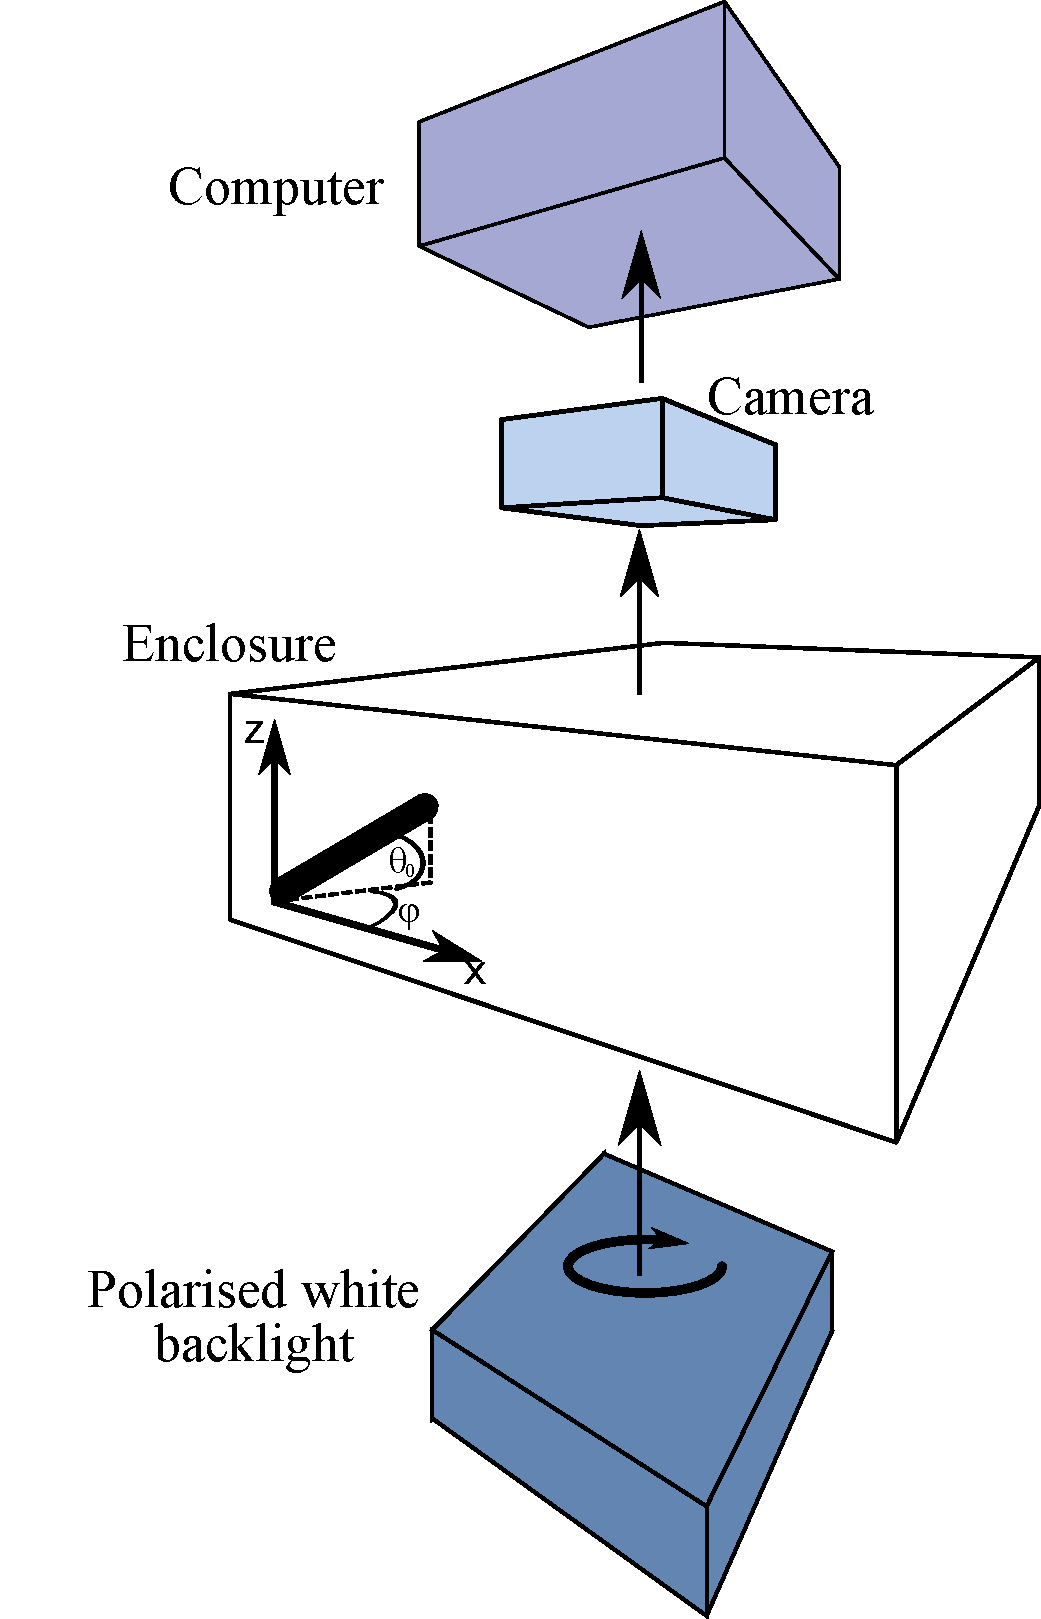
\includegraphics[width=0.3\textwidth]{Figures/Pretilt/camera_kit}
\end{center}
\caption[Schematic diagram of machine vision setup]{\label{fig:camerakit}Schematic diagram of the machine vision technique of measuring surface pretilt. A polarised white back light is shone through the enclosure containing the anti-parallel dye-doped cells, before passing into a camera and computer for analysis.}
\end{figure}
\subsection{Experiment}

\subsection{Over-baked Nissan SE-1211 recipe}
\label{sec:1211recipe}
3.2 cm by 2.5 cm glass slides with a conductive Indium Tin Oxide (ITO) coating on one side were spin coated at 4000 RPM for 40 seconds with the vertical aligning polyimide Nissan SE-1211. They were coated on either the plain glass side or on the ITO side. This allowed for the production of complete cells with either ITO or plain glass on the inner bounding surfaces.

After the Nissan SE-1211 aligning layer was deposited, the slides were pre-baked at 95 $^\circ$C for 1 minute on a hotplate, prior to being baked in an oven at 240 $^\circ$C for 60 minutes. This baking temperature is far above the manufacturer's guidelines of 180 $^\circ$C for 50 minutes \cite{Wang2007}, hence the term `over-baked' Nissan SE-1211. As suggested in Section \ref{sec:over-baked}, it is this over-baking process that plays the important role in producing pretilt angles away from what would conventionally be a vertical aligning surface. 

On removal from the oven, the slides were rubbed via a moving stage passing under a spinning drum with a rubbing cloth attached around the circumference as shown in Figure \ref{fig:rubbingmachine}. The rubbing system is set up so that the height of the stage can be varied from a level where the slides are made to pass under the drum barely touching the surface of the cloth, up to close contact between the slide and the cloth. It is important to note here that several authors have tried to quantify the strength of rubbing when referring to a rotating drum moving over the surface of a sample \cite{Wang2007, Huang2005,Vaughn2007,Pidduck1996}. In this case, it is believed that the quantification of a rubbing strength parameter is dependent on too many variables and will be very difficult to reproduce exactly on another experimental setup. In these experiments, as we are showing only general trends in the degree of pretilt as function of this rubbing strength, we define simply a rubbing height $d$, that can vary from 3.8 mm (strongest contact with the slide) to 4.5 mm (weakest contact with the slide). The experimental rubbing machine parameters are also shown in Figure \ref{fig:rubbingmachine}.

\begin{figure}
\begin{center}
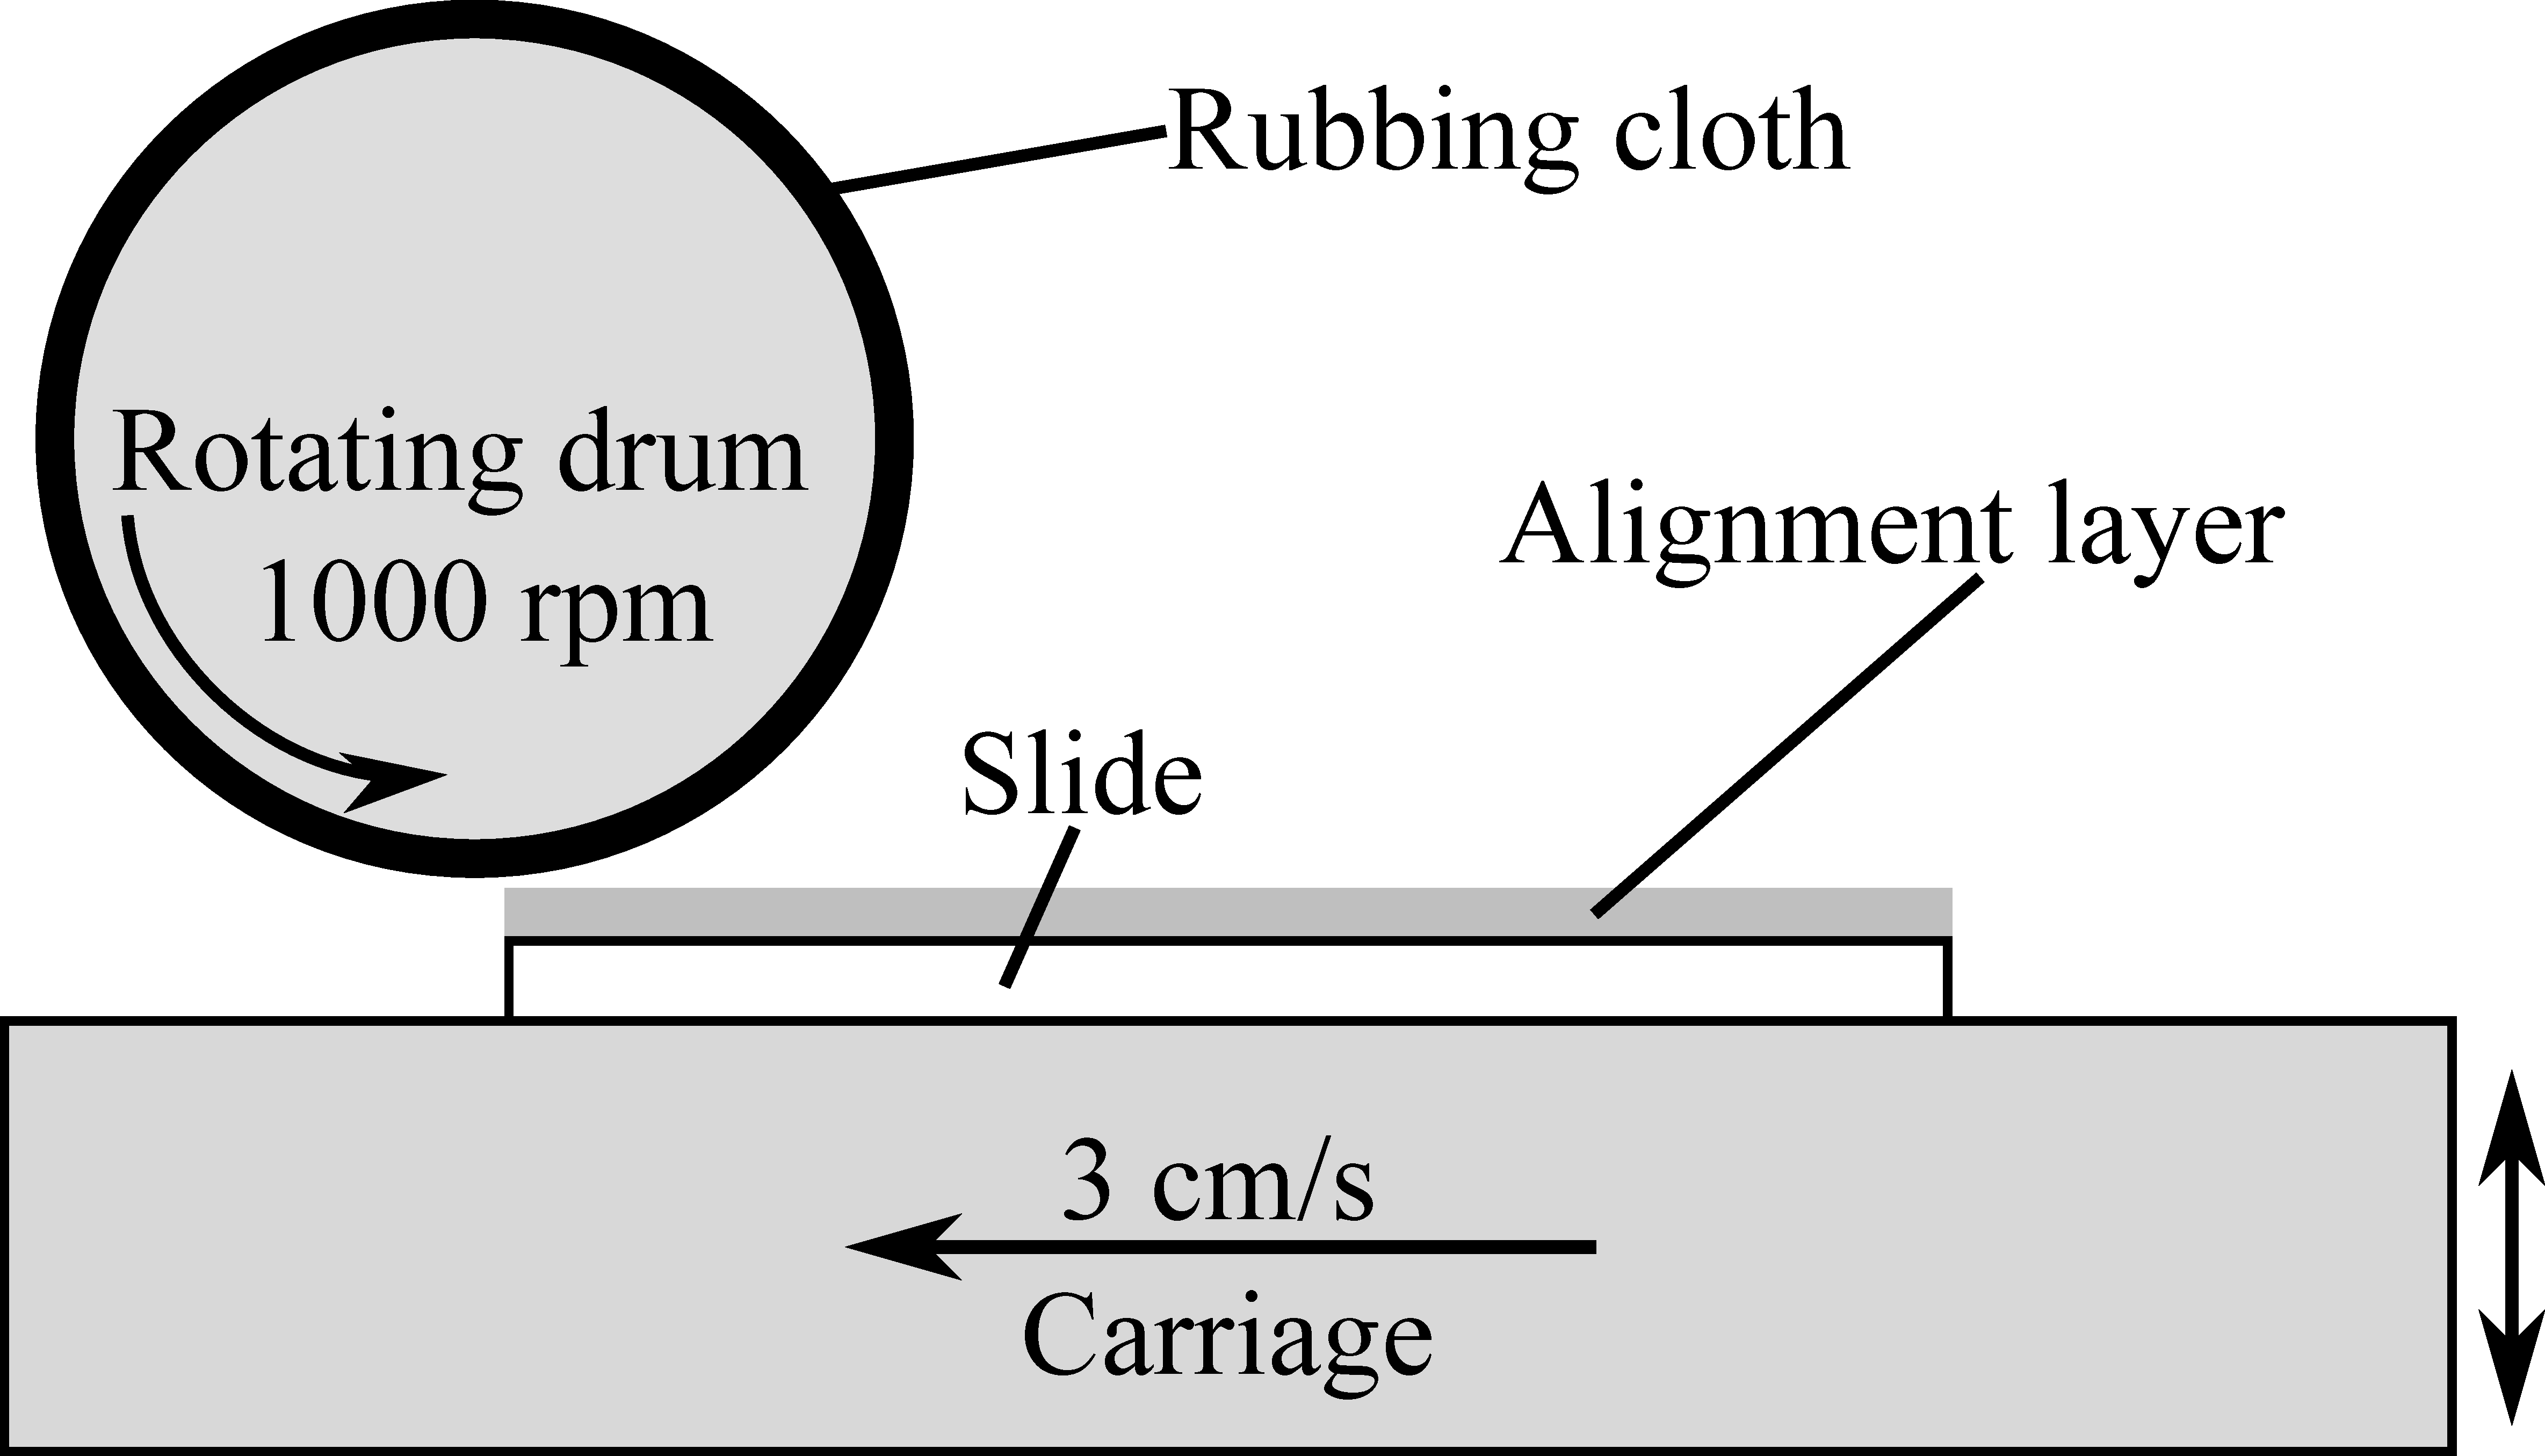
\includegraphics{Figures/Pretilt/rubbing_machine}
\end{center}
\caption[Schematic diagram of rubbing machine]{\label{fig:rubbingmachine}A schematic representation of the experimental rubbing machine set up. The moving carriage with sample attached are passed under the rotating drum and rubbing cloth at varying strengths of contact. To vary the rubbing strength, the carriage can be moved up or down.}
\end{figure}

After both the plain glass and ITO coated glass slides were rubbed at varying values of $d$, liquid crystal cells were fabricated by aligning the top and bottom plates in an anti-parallel geometry (with no twist gradient in $z$), creating a uniformly\footnote{Provided both surfaces have been treated identically, as will be discussed in the analysis (Section \ref{sec:pretilt_analysis})} tilted slab of liquid crystal between the top and bottom surfaces. The cells were spaced with 5 $\mu$m beads dispersed in a UV curing glue (Norland optical adhesive 73). The cells were then capillary filled in the isotropic phase with 5CB doped with 1\% by weight of each of G472, G241 and G232 dichroic dyes from Hayashibara for use in measuring the pretilt angle as described in Section \ref{camerakit}.


\subsection{Over-baked Nissan SE-1211 results}
\label{sec:1211_results}
Figure \ref{fig:ito_glass} shows a plot of the measured pretilt angle as a function of both the rubbing parameter, $d$, and the surface type upon which the Nissan SE-1211 is deposited (ITO or glass). The first observation to make is that for both sets of data, the pretilt angle (measured from the surface normal) increases as we increase the rubbing strength (a decrease in $d$). Qualitatively, this suggests that the harder we rub the surface of the over-baked vertical layer, the further the aligning molecules are distorted from their original vertical state, becoming more planar.

For both surfaces there is the suggestion of a threshold, below which, any weaker rubbing results in little or no deformation away from the minimum pretilt angle measured (it is important to note here that a pretilt angle of $\theta_0\approx0^{\circ}$ would be achieved just by conventionally treated Nissan SE-1211, with no mechanical rubbing of the surface). This threshold is shown by the saturation of the pretilt angle when the surface is rubbed weakly ($d=4.4$ and $d=4.5$ for both glass and ITO coated glass) in Figure \ref{fig:ito_glass}. For Nissan SE-1211 spun onto the ITO coated glass surface, this value is approximately $5^{\circ}$ (or $85^{\circ}$ tilted away from the surface) and for the case of Nissan SE-211 coated onto the glass surface, the value is slightly lower (approximately $20^{\circ}$, or $70^{\circ}$ away from the surface). This result is not wholly unexpected, and qualitatively it agrees very well with the results obtained by Rosenblatt \textit{et al.} \cite{Huang2005}, where a threshold rubbing strength is observed before the onset of distortion of the director away from vertical alignment (detailed in Section \ref{sec:over-baked}). The similarity of these results is considered here to be purely qualitative, due to the ill-defined variable of a rubbing strength. However, the finding does go some way in confirming the phenomenon of a threshold rubbing strength for pretilt in over-baked Nissan SE-1211 aligning layers.

It is also shown in Figure \ref{fig:ito_glass} that the lowest value of the pretilt angle is not $0^{\circ}$ (particularly in the case of Nissan SE-1211 spun onto glass), which we would perhaps have expected from a conventionally treated Nissan SE-1211 polyimide alignment layer. This result again occurs at the weakest rubbing strengths and suggests that the over-baking process could be responsible for the small deviation of the director away from vertical alignment. It is likely that this pretilt angle occurs in randomly oriented domains as has been observed by Wang \textsl{et al.} \cite{Wang2007}, and in this case, the rubbing process gives an overall azimuthal alignment direction as well as further increasing the deformation of the director at the surface.

\begin{figure}
\begin{center}
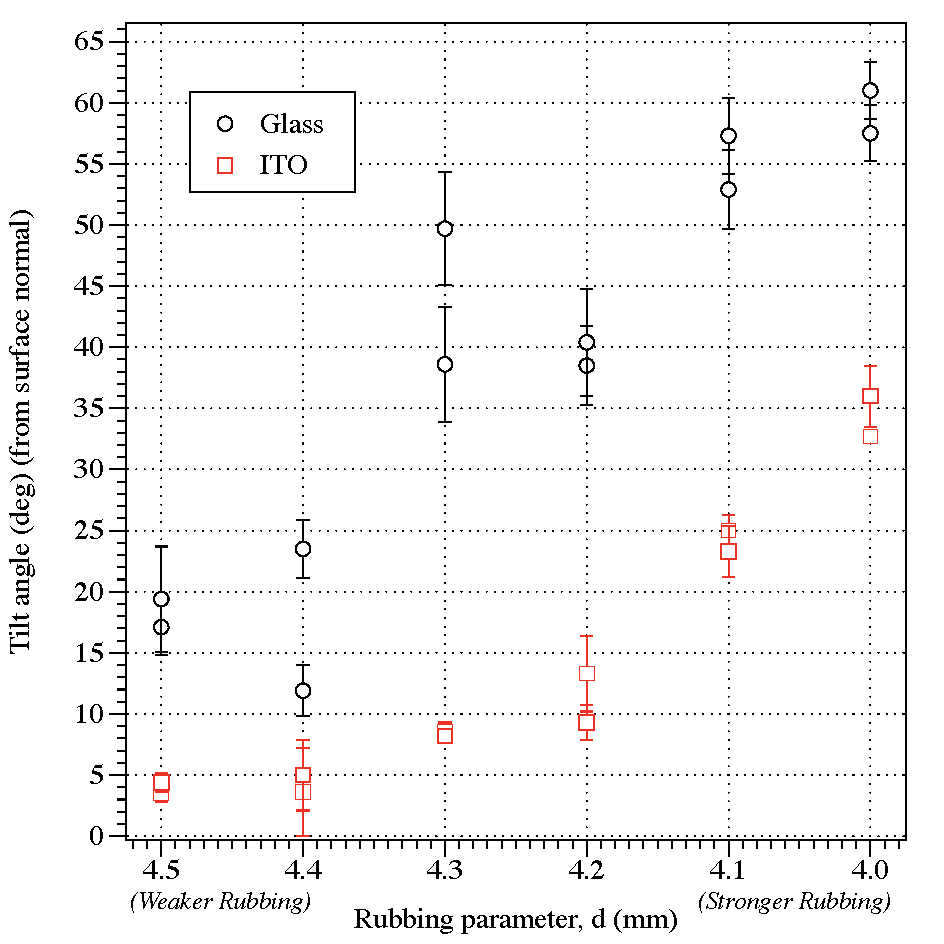
\includegraphics{Figures/Pretilt/ito_glass}
\end{center}
\caption[Pretilt angle as a function of rubbing parameter for glass and ITO surfaces]{\label{fig:ito_glass}{Measured pretilt angle as a function of the rubbing parameter for the over-baked Nissan SE-1211 aligning layer. Results show a clear difference for cells prepared with the aligning layer on ITO and glass.}}
\end{figure}

Perhaps the most interesting feature of Figure \ref{fig:ito_glass}, is that the measured pretilt angle is higher in the case of Nissan SE-1211 spun onto the plain glass surface than for the Nissan SE-1211 spun onto the ITO coated glass surface, for all values of the rubbing parameter. It is clear that the director is closer to vertical alignment for samples prepared on ITO coated glass, rather than that of plain glass, for any given value of the rubbing parameter. In the case of samples prepared on glass, the pretilt angle is shown to be tuneable from approximately $20^{\circ}$ to $60^{\circ}$, whereas for samples prepared on ITO coated glass, the pretilt angle is tuned from approximately $5^{\circ}$ to $35^{\circ}$ for the same values of the rubbing parameter. The error bars shown in Figure \ref{fig:ito_glass} are calculated from the standard deviation in the pretilt measurement across several areas of the cell and give a measure of the magnitude of the spatial variability in pretilt produced by this procedure. In both cases of glass and ITO coated glass, a surface profiling experiment has shown that the thickness of the Nissan SE-1211 aligning layer is very similar (layer thickness of approximately 170 nm on glass and 180 nm on ITO coated glass) at a spin rate of 4000 rpm, shown in Figure \ref{fig:scratch}. The aim of this measurement is to see whether or not the surface upon which the polymer is deposited plays an important role in the thickness of the aligning layer, and ultimately, whether it has an effect on the degree of pretilt created. The result shown in Figure \ref{fig:scratch}, indicating the similar thicknesses, goes a long way to removing any doubt about the difference in pretilt measured for glass and ITO coated glass being the result of a difference in the aligning layer thickness. 

Figure \ref{fig:cells} shows an optical photograph of over-baked Nissan SE-1211 cells fabricated using this recipe. The cells (containing the dichroic dye) are placed on a polarised back light and ordered with respect to surface type and rubbing parameter, with the cell's rubbing direction parallel to the light's incident electric field. It is clear that as the rubbing strength is increased, the cells become darker (as the dichroic dye is absorbing more light), implying that the director is gradually tilting further away from vertical alignment. As is also shown by the pretilt measurement of the camera kit in Figure \ref{fig:ito_glass}, the glass cells in Figure \ref{fig:cells} are darker than the ITO coated glass cells, confirming by eye, the existence of different pretilt responses for over-baked and rubbed Nissan SE-1211 alignment layers coated on both glass and ITO coated glass.

Some preliminary experiments have also shown that a similar trend of stronger rubbing producing more planar alignment is also observed for over-baked Nissan SE-1211 cells filled with the liquid crystal ZLI-2293 (Merck).



\begin{figure}
\begin{center}
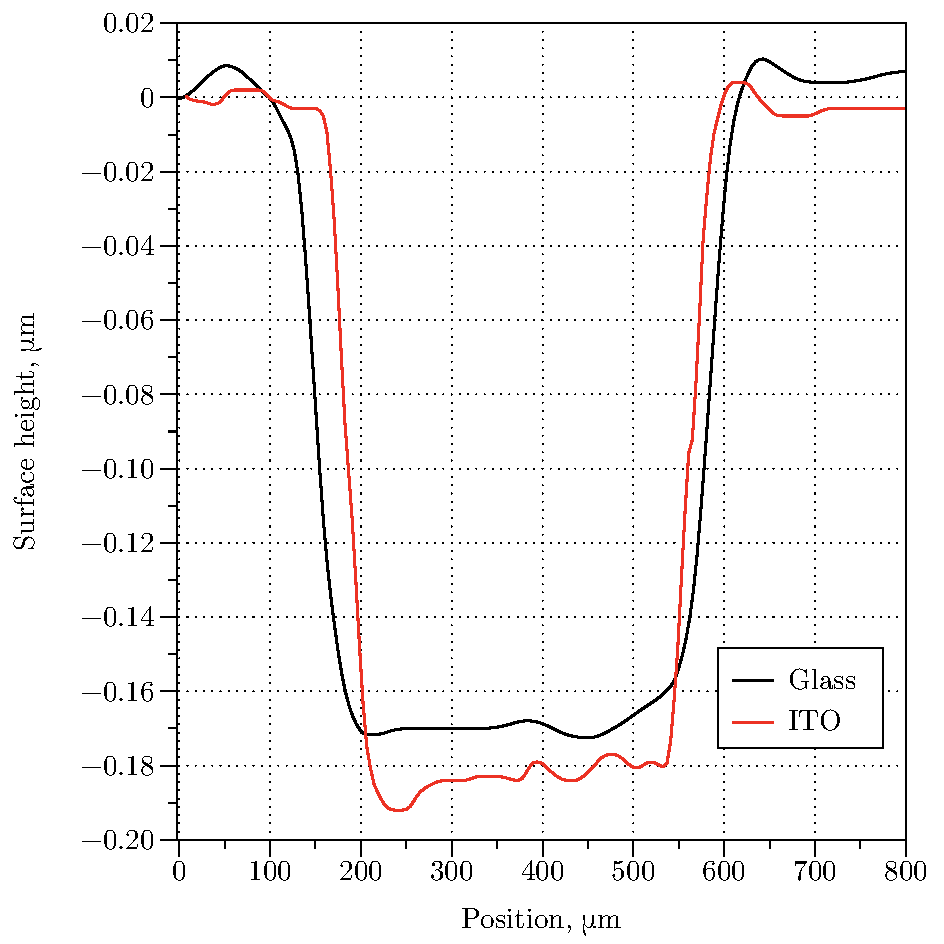
\includegraphics{Figures/Pretilt/scratch}
\end{center}
\caption[Surface profile of scratched aligning layers]{\label{fig:scratch}{Surface profile of a scalpel scratch made in the Nissan SE-1211 aligning layer spun onto glass and ITO coated glass substrates as detailed in Section \ref{sec:1211recipe} at a rate of 4000 rpm. This figure suggests that the depth of the polyimide layer is very similar on both surfaces, approximately 170 nm on Glass and 180 nm on ITO coated glass.}}
\end{figure}

\begin{figure}
\begin{center}
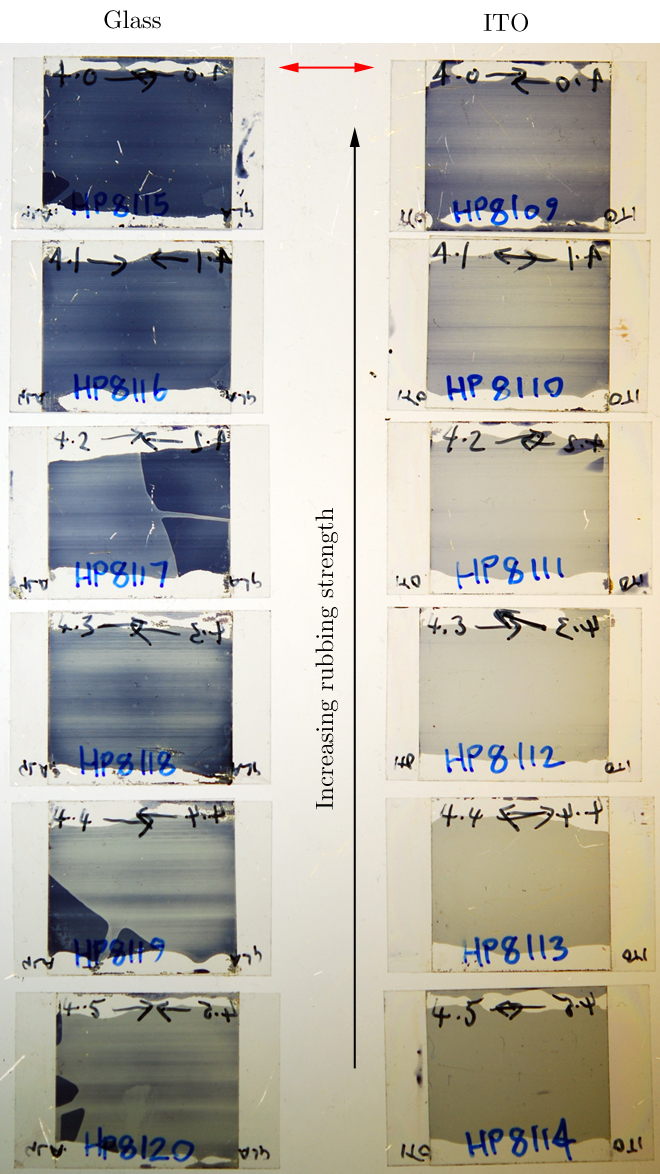
\includegraphics{Figures/Pretilt/cells}
\end{center}
\caption[Photograph of cells fabricated using over-baked Nissan SE-1211]{\label{fig:cells}{A photograph of the over-baked Nissan SE-1211 cells. The cells on the left have the aligning layer deposited on the glass side whilst the cells on the right have the aligning layer deposited on the ITO side. The rubbing strength increases from the bottom of the image to the top (ranging from 4.5 to 4.0). Cells that have been rubbed harder are noticeably darker (more planar), with the glass cells being darker than the ITO cells}. The polarisation of the back light is indicated by the red arrow (parallel to the rubbing direction).}
\end{figure}

\subsection{Contact angles and surface energies}
As a further investigation into the ability of over-baked Nissan SE-1211 layers to produce intermediate pretilt angles, the surface energies of the alignment layer were measured as a function of the rubbing parameter, where the alignment layers were prepared identically to those described previously in Section \ref{sec:1211recipe}.

The contact angle of a droplet on a surface and the subsequent surface energy of the aligning layer has long been a method employed to obtain useful information about the alignment properties of that layer. This method of measuring the surface energy, through the contact angle of a droplet on the surface, is often used due to it's speed and ease of implementation. However, whether or not the surface energy of an aligning layer reveals any information about the ability of the surface to promote vertical or planar alignment, seems to be unclear \cite{Cognard1982}. In some systems, liquid crystal alignment does definitely appear to have a strong correlation to the surface energy \cite{Hwang2010} of the alignment layer, in others, as we shall see here, the link is not so clear.

In this study, the substrates were spin coated and rubbed, but not made into complete cells. They were left as free surfaces, in order to place a droplet of liquid on the polymer layer and measure the contact angle created. Surfaces were again coated with over-baked Nissan SE-1211 on either the plain glass side or the conductive ITO coated glass side. This again allows us to see if there is any difference in the surface energy as a function of both the surface that the polymer is coated on and the rubbing strength.

The contact angles were measured using a Cam 200 contact angle goniometer (KSV Instruments) \cite{Cammanual} by placing droplets of water, ethylene glycol and di-iodemethane onto the coated and rubbed substrate. A digital camera was then used to capture images of the drop a few seconds after it had been dispensed, allowing the contact angle between the drop and the surface to be measured (via a computer spline fit to the drop's surface), as is shown in Figure \ref{fig:contact_angles}. These contact angles were then used to calculate the Owens, Wendt, Rabel and Kaelble (OWRK) surface energies \cite{Owens1969}.

\begin{figure}
\begin{center}
\subfigure[]{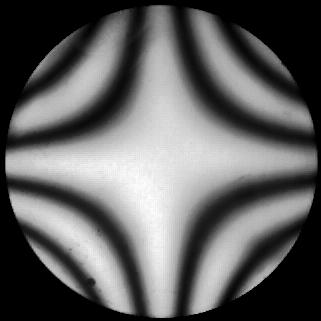
\includegraphics[width=0.15\textwidth]{Figures/Pretilt/Contact_angle/0.jpg}}
\subfigure[]{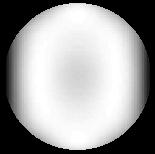
\includegraphics[width=0.15\textwidth]{Figures/Pretilt/Contact_angle/1.jpg}}
\subfigure[]{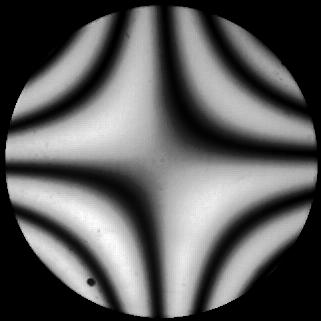
\includegraphics[width=0.15\textwidth]{Figures/Pretilt/Contact_angle/2.jpg}}
\subfigure[]{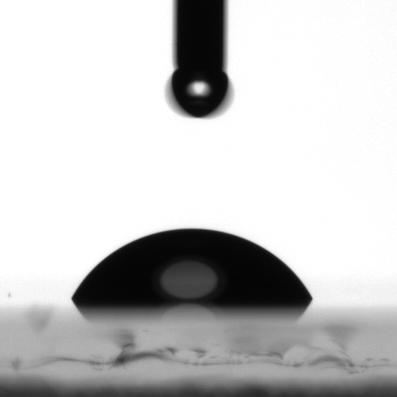
\includegraphics[width=0.15\textwidth]{Figures/Pretilt/Contact_angle/3.jpg}}
\subfigure[]{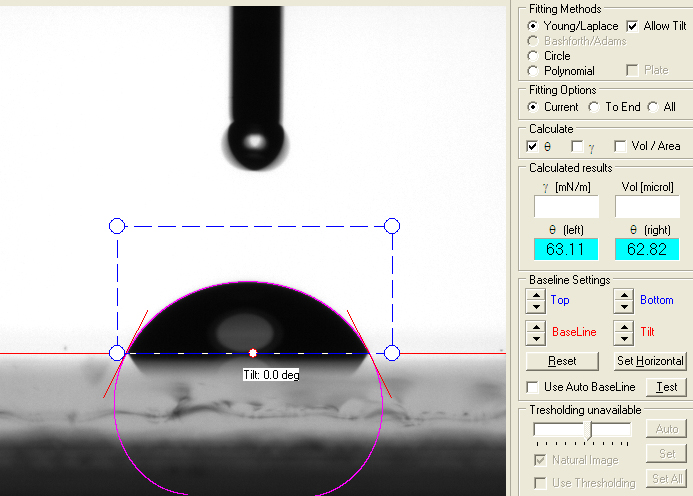
\includegraphics[width=0.48\textwidth]{Figures/Pretilt/Contact_angle/fit.jpg}}
\end{center}
\caption[Droplet dispensing for contact angle measurement]{\label{fig:contact_angles}Figures (a) to (d) show optical photographs of the droplet dispensing technique. The droplet is formed at the end of the syringe (a), moved down to contact the surface (b), pulled away (c) and then left to stabilise (d). Figure (e) shows the fit and measurement of the contact angle made by the bespoke software.}
\end{figure}

\subsection{OWRK surface energies}
\label{sec:owrk}
The Owens, Wendt, Rabel and Kaelble (OWRK) technique, is a method that resolves the approximate surface energy of an aligning layer into contributions from both the dispersive and dipole-hydrogen bonding forces of the droplet on the surface. It is noted in reference \cite{Owens1969} that this method is particularly applicable to the characterisation of polymer surface energies, as are being examined in this chapter. 

\subsection{OWRK equation derivation}
As is carried out in the experiment, the OWRK surface energy is calculated from the contact angle $\beta$ created by a liquid droplet upon the surface of a polymer. In this system, each of the phases involved, the polymer (solid, $s$) and the droplet (liquid, $l$), can be split (in the OWRK method) into both polar $p$, and disperse $d$, fractions. Therefore, the surface energies of the solid and liquid phases respectively can be written as,

\begin{eqnarray}
\sigma_l=\sigma_l^p+\sigma_l^d\\
\sigma_s=\sigma_s^p+\sigma_s^d
\end{eqnarray}

Where $\sigma$ denotes the surface energy, subscript letters represent the phase type (solid $s$, or liquid $l$) and superscript letters represent the fraction of the surface tension (polar $p$, or disperse $d$). Owens and Wendt took the equation for the surface tension,

\begin{equation}
\gamma_{sl}=\sigma_s+\sigma_l-2\left(\sqrt{\sigma_s^d\sigma_l^d}+\sqrt{\sigma_s^p\sigma_l^p}\right)
\label{eq:surface_tension}
\end{equation}

\noindent and combined it with the Young equation,

\begin{equation}
\sigma_s=\gamma_{sl}+\sigma_l\cos{\left(\beta\right)}
\label{eq:young}
\end{equation}

\noindent to yield (by substitution of equation \ref{eq:young} into equation \ref{eq:surface_tension}),

\begin{equation}
\sigma_s-\left(\sigma_l\cos{\left(\beta\right)}\right)=\sigma_s+\sigma_l-2\left(\sqrt{\sigma_s^d\sigma_l^d}+\sqrt{\sigma_s^p\sigma_l^p}\right)
\end{equation}

\noindent and rearranging  for the familiar $y=mx+c$ linear form,

\begin{equation}
\frac{\left(1+\cos{\left(\beta\right)}\right)\sigma_l}{2\sqrt{\sigma_l^d}}=\sqrt{\sigma_s^p}\sqrt{\frac{\sigma_l^p}{\sigma_l^d}}+\sqrt{\sigma_s^d}
\label{eq:owrk}
\end{equation}

In this experiment, the contact angles created between droplets of water, ethylene glycol, di-iodemethane and the polymer alignment layer are measured, and subsequently converted into surface energies by calculation of the gradient of equation \ref{eq:owrk}, where explicitly, $\beta$ is the contact angle between the droplet and the surface, $\sigma_l$ is the total surface tension of the liquid, $\sigma_l^d$ is the disperse component of the liquid surface tension, $\sigma_l^p$ is the polar component of the liquid surface tension, $\sigma_s^d$ is the disperse component of the polymer surface tension and $\sigma_s^p$ is the polar component of the surface. The test-liquid surface tensions used for these calculations are given in Table \ref{tab:owrk}.

By plotting
\begin{equation}
\frac{\left(1+\cos\left(\beta\right)\right)\sigma_l}{2\sqrt{\sigma_l^d}} \text{\hspace{0.7mm} vs \hspace{0.7mm}} \sqrt{\frac{\sigma_l^p}{\sigma_l^d}}
\end{equation}

the gradient, $\sqrt{\sigma_s^p}$ and $y$-intercept $\sqrt{\sigma_s^d}$ allow us to measure the polar and disperse components of the polymer's surface energy, as is shown in Figure \ref{fig:owrk} for a glass surface rubbed at $d=4.2$. The surface energy is shown to be approximately 40.6 mJ/m$^2$.

\begin{figure}
\begin{center}
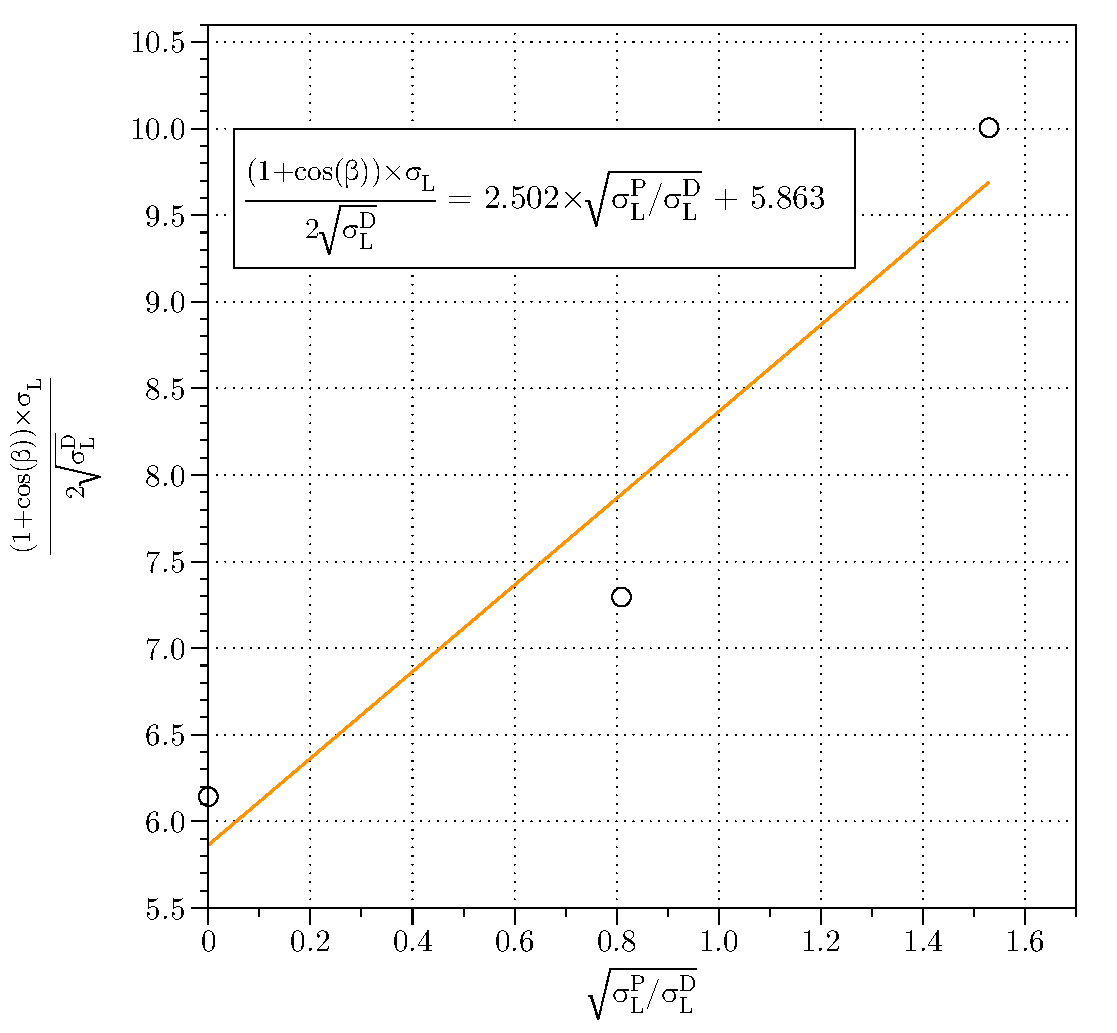
\includegraphics{Figures/Pretilt/owrk}
\end{center}
\caption[Calculation of surface energies]{\label{fig:owrk}{A linear fit to the data points gives the value of the gradient, $\sqrt{\sigma_s^p}=2.5$, intercept, $\sqrt{\sigma_s^d}=5.9$ and subsequently the polar, $\sigma_s^p=6.2$ mJ/m$^2$, disperse, $\sigma_s^d=34.4$ mJ/m$^2$ and total, $\sigma_s^t=40.6$ mJ/m$^2$ components of the polymer surface energy. In this case, the surface energy is calculated for Nissan SE-1211 coated on glass and rubbed at a value of $d=4.2$}}
\end{figure}

\subsection{Surface energy results}

Figure \ref{fig:contact_angles/energies} shows the contact angle $\beta$ and surface free energies $\sigma$ for the over-baked Nissan SE-1211 recipe. The contact angles are shown as a function of the rubbing height and the test liquid used to make the droplet, along with the calculated OWRK surface energies. Figure \ref{fig:contact_angles/energies} (a) shows how the contact angles measured for over-baked Nissan SE-1211 on the glass surface vary as a function of the rubbing parameter and test drop (water, ethylene glycol and di-iodomethane). It is seen that the contact angles vary very little across the majority of rubbing strengths, except for $d=4.0$ (strongest rubbing), here we see a rise in the contact angle which is most likely due to mechanical damage of the aligning layer caused by the strong rubbing (sometimes scratches can be seen in the aligning layer at particularly hard rubbing strengths). Figure \ref{fig:contact_angles/energies} (c) shows how the value of the surface energies also seem to vary little across the range of rubbing strengths used for Nissan SE-1211 coated on the glass surface, except for at $d=4.0$. This result is unsurprising due to the method of surface energy calculation, described in Section \ref{sec:owrk}. Figures \ref{fig:contact_angles/energies} (b) and (d) depict the same information for the Nissan SE-1211 on the ITO coated glass surface. Here we see a similar result as for the Nissan SE-1211 on glass, with very little difference in the contact angles and surface energies as a function of the rubbing strength, except for at $d=4.0$. Perhaps most importantly, the calculated surface energies differ very little between the glass surface and the ITO coated glass surface with $\bar{\sigma}_{g}=39.9 \pm 1.6$ mJ/m$^2$ and $\bar{\sigma}_{ITO}=36.1\pm1.3$ mJ/m$^2$, leading to the conclusion that the measured surface energies give little or no information regarding the manner in which the surface treatment controls the degree of pretilt exhibited in a cell.


\begin{table}[ht]
\centering  % used for centering table
\begin{tabular}{c c c c} 
\hline\hline                       
Surface tension (mN/m)	&Water 	&Ethylene Glycol		&Di-iodomethane\\
\hline                  
Total					& 72.8	& 48				& 50.8\\
Disperse				& 21.8	& 29				& 50.8\\
Polar					& 51	  	& 19				& 0\\ 
\hline
\end{tabular}
\caption{OWRK test liquid parameters} 
\label{tab:owrk}
\end{table}


\begin{figure}
\begin{center}
\subfigure[Glass contact angles]{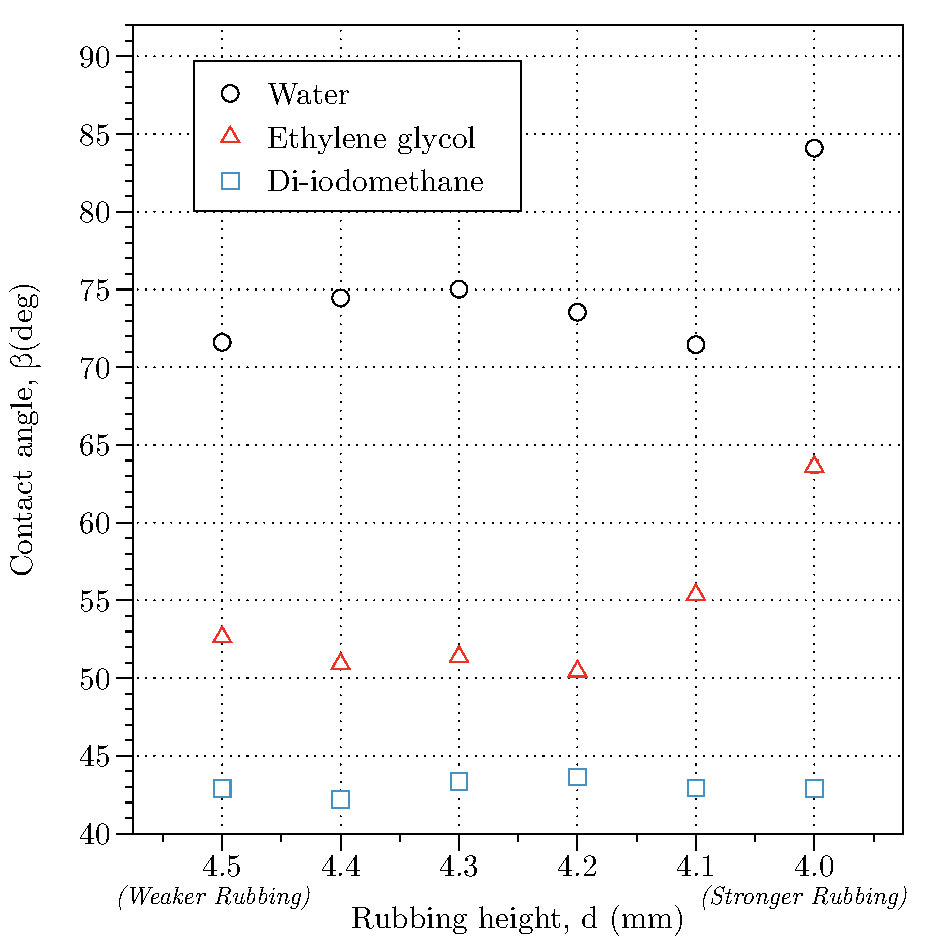
\includegraphics[width=0.25\textwidth]{Figures/pretilt/glass_contact}}
\subfigure[ITO contact angles]{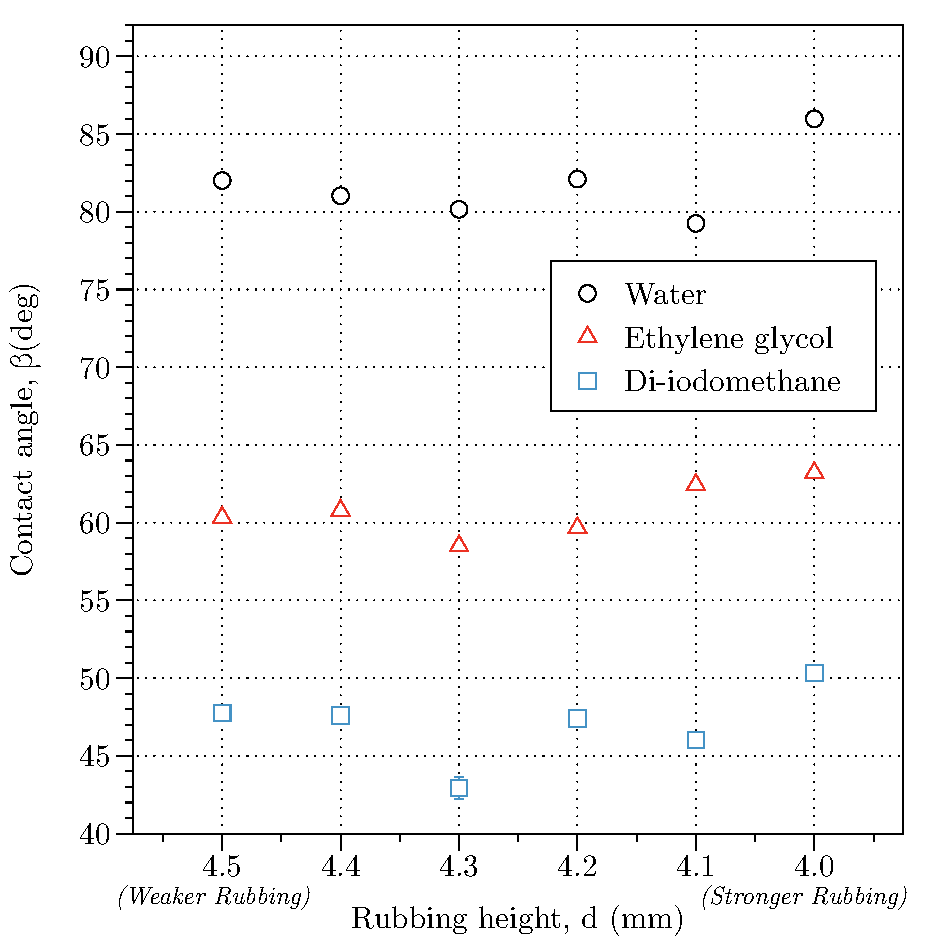
\includegraphics[width=0.25\textwidth]{Figures/pretilt/ito_contact}}
\subfigure[Glass surface energies]{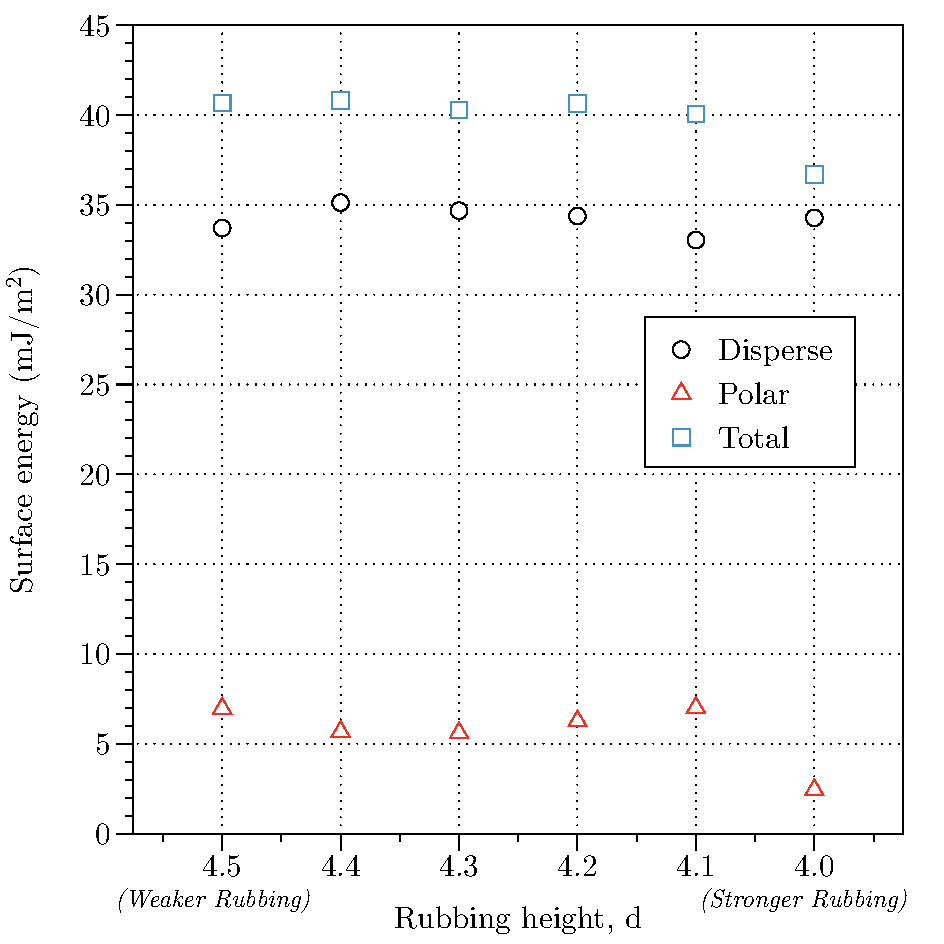
\includegraphics[width=0.25\textwidth]{Figures/pretilt/glass_energy}}
\subfigure[ITO surface energies]{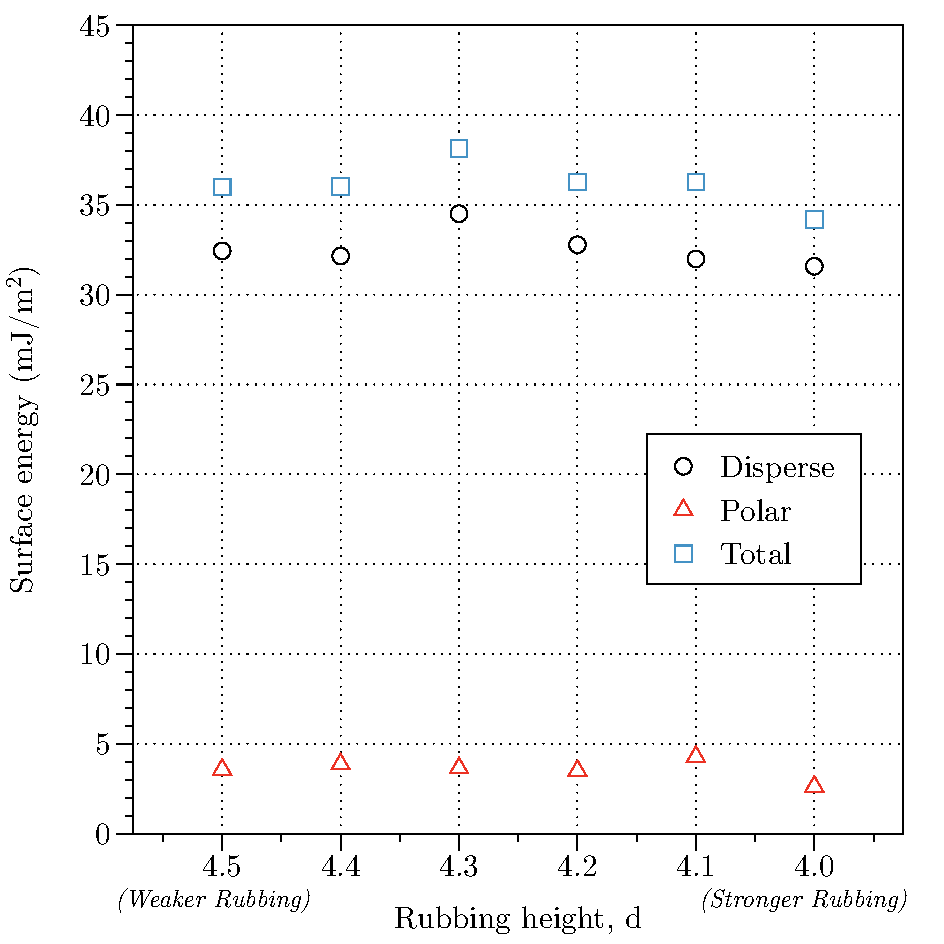
\includegraphics[width=0.25\textwidth]{Figures/pretilt/ito_energy}}
\end{center}
\caption[Contact angles and surface energies]{\label{fig:contact_angles/energies}Contact angles and surface energies for droplets of water, ethylene glycol and di-iodomethane as a function of the rubbing strength on over-baked Nissan SE-1211 polyimide layers. (a,b) Contact angles on glass and ITO. (c,d) Surface energies for glass and ITO.}
\end{figure}

\subsection{Bi-layer polyimide recipe}
\label{sec:double_layer}

ITO coated glass slides are spin coated (on the ITO coated side) with the vertical aligning polyimide Nissan SE-4811 at 4000 rpm for 40 seconds. The samples are then pre-baked on a hotplate at 100 $^{\circ}$C for 10 minutes, before being baked in an oven at 210 $^{\circ}$C for 40 minutes. After curing, a planar aligning layer of Nissan SE-130 is spin coated on top of the vertical Nissan SE-4811 aligning layer, at spin rates that range from 3000 to 4000 rpm. The sample is then pre-baked on a hotplate at 100 $^{\circ}$C for 10 minutes and finally fully cured in an oven at 210  $^{\circ}$C for 40 minutes. For these experiments, two slides were not coated with the Nissan SE-130 layer, in order to build a control cell with just a vertical Nissan SE-4811 surface alignment layer.

The slides are then rubbed at varying strengths (using the same rubbing parameter $d$, as per the over-baked Nissan SE-1211 recipe) and constructed into liquid crystal cells. The cells were again fabricated by aligning the top and bottom plates in an anti-parallel geometry, spaced with 5 $\mu m$ beads dispersed in a UV curing glue. The cells were then capillary filled in the isotropic phase with ZLI-2293 (Merck) doped with the same dichroic dyes as used before in Section \ref{sec:1211recipe}. The high throughput camera kit technique was then used to measure the degree of pretilt exhibited in each cell.

\subsection{Bi-layer polyimide results}
Figure \ref{fig:double_polyimide} shows the measured pretilt angle for the double polyimide recipe as a function of both the rubbing strength and Nissan SE-130 (planar aligning) spin rate for anti-parallel cells filled with ZLI-2293. Firstly, it is shown that for the control sample (purple data point) for which no planar aligning layer was coated on top of the base vertical layer, the measured value of the liquid crystal tilt angle is close to vertical (as we would have expected from a conventional Nissan SE-4811 aligning layer) even though in this case it has been rubbed moderately hard $\left(d=4.0\right)$. This result is interesting in itself, as a layer of the over-baked vertical aligning Nissan SE-1211 has shown significant distortion away from vertical alignment when rubbed at $d=4.0$ as is shown in Figure \ref{fig:ito_glass} for alignment on surfaces of glass and ITO coated glass. This may lend some strength to the argument that the over-baking process itself (for Nissan SE-1211) has an effect on weakening the alignment axis of the polymer backbone. 

For the sample where a layer of Nissan SE-130 is spun at 3500 rpm on top of the already coated Nissan SE-4811 layer (black data points), there is a clearly linear trend in the pretilt angle with respect to the rubbing strength. This trend is maintained over all rubbing strengths used, and shows that the value of the pretilt angle can be varied from approximately $3^{\circ}$ to $24^{\circ}$. It is worth noting that although the samples in this experiment are rubbed over a similar range of strengths as those in the over-baked Nissan SE-1211 experiment (Section \ref{sec:1211recipe}), the range of pretilt angles achieved here are much smaller. This difference could be due to the use of the liquid crystal ZLI-2293 as opposed to 5CB, in addition to the difference in the recipes. 

Figure \ref{fig:double_polyimide} also shows pretilt angle measurements for Nissan SE-130 alignment layers spun at rates of 3000 and 4000 rpm, which within error, give very similar pretilt values of close to 10$^{\circ}$. This leads to the conclusion that for this sample set, there is no real trend in the pretilt angle as a function of the Nissan SE-130 alignment layer spin rate. Zheng \text{et al.} \cite{Zheng2007} have shown that the degree of pretilt can be tuned all the way from vertical to planar in samples filled with the liquid crystal E7 (main component 5CB), where the Nissan SE-130 layer and it's subsequent thickness is the controlling variable. Here we have seen that the Nissan SE-130 aligning layer thickness has little measurable effect on the degree of pretilt created.

\begin{figure}
\begin{center}
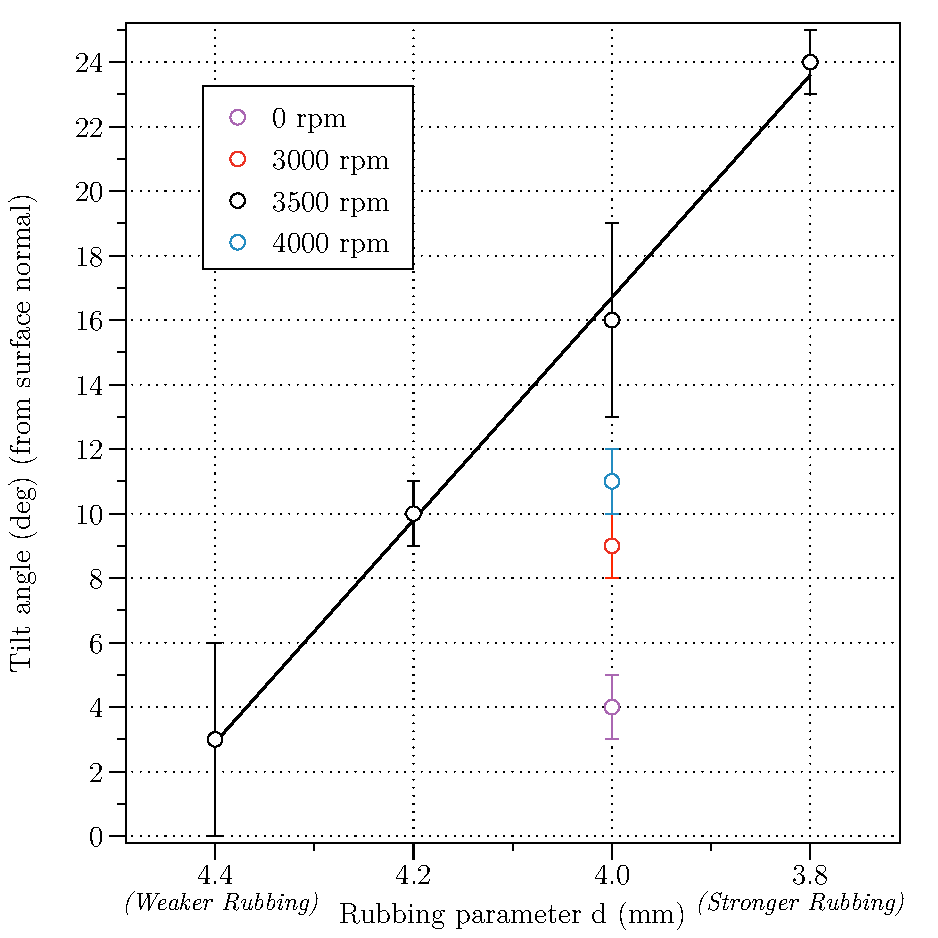
\includegraphics{Figures/Pretilt/double_polyimide}
\end{center}
\caption[Pretilt angle as a function of rubbing parameter]{\label{fig:double_polyimide} Measured pretilt angle as a function of the rubbing parameter $d$, and Nissan SE-130 (planar aligning) spin rate.}
\end{figure}

In order to truly test the double polyimide recipe's ability to produce intermediate pretilt angles, further experiments were carried out using the liquid crystals 5CB and E7. Our measurements on cells filled with 5CB and E7 showed by eye that alignment of the liquid crystal was very near to, or was indeed vertical, for all Nissan SE-130 spin rates. However it is worth noting that spin coating the Nissan SE-130 on top of the baked Nissan SE-4811 almost always leads to a non-uniform coverage of the Nissan SE-4811 surface. This can be seen after the spinning process, where it appears that the Nissan SE-130 layer forms droplets on the surface and there are only patches of coverage. Some other preliminary experiments have shown that an oxygen plasma ash treatment (as is standard in many semiconductor research facilities) of the baked Nissan SE-4811 layer before applying the Nissan SE-130 layer can significantly reduce this effect, presumably because the Nissan SE-130 is better able to wet the Nissan SE-4811 layer. For cells where the Nissan SE-4811 layer is given the oxygen plasma ash treatment, we have seen some moderate pretilt for the liquid crystal 5CB, with values of approximately 30$^{\circ}$, but still no clear trend with respect to the Nissan SE-130 spin rate (shown in Figure \ref{fig:double_polyimide_5cb}). Figure \ref{fig:double_polyimide_5cb} also demonstrates the temporal robustness of the induced pretilt from the double polyimide recipe. The black and red data points are taken 20 days apart yet show very similar values of tilt angle (small discrepancies may appear from spatial inhomogeneities in the pretilt angle and a small error in reproducing the measurement from exactly the same area of the cell). 

\begin{figure}
\begin{center}
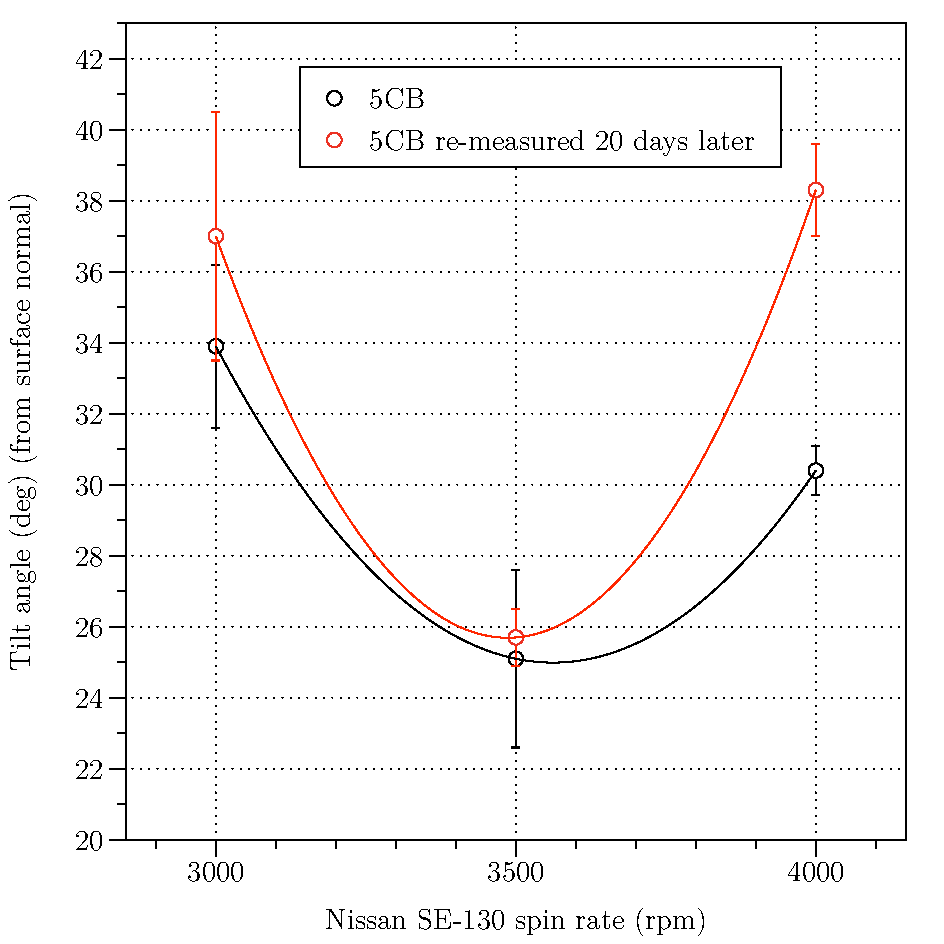
\includegraphics{Figures/Pretilt/double_polyimide_5cb}
\end{center}
\caption[Pretilt angle as a function of rubbing strength for 5CB]{\label{fig:double_polyimide_5cb} Measured pretilt angle as a function of the Nissan SE-130 spin rate for cells filled with 5CB. The red data points show the same measurement made 20 days after the original (black data points).}
\end{figure}

\subsection{Analysis/Conclusions}
\label{sec:pretilt_analysis}

In this chapter, two methods for varying the degree of surface pretilt exhibited at the bounding surface of a liquid crystal cell have been characterised. The first recipe, over-baked and rubbed Nissan SE-1211, has shown results that share a similar trend to that of Rosenblatt \textit{et al.} \cite{Wang2007,Huang2005}, but here we observe that the surface upon which the aligning polyimide is deposited plays a crucial role in the magnitude of the pretilt angle measured. It has been shown in Figure \ref{fig:ito_glass} that the pretilt angles are consistently lower for cells where the Nissan SE-1211 is coated onto the plain glass side rather than onto the ITO coated glass side. The reason for this observation is still unclear, with surface profiling experiments (Figure \ref{fig:scratch}) showing that the polyimide layer thickness is similar for both cases. One possible suggestion is that the conductive nature of the ITO surface plays a role in removing static charge from the surface, or at least modifies the local electric field, which is without doubt present in the rubbing process. For both surfaces, there is also a threshold for the onset of pretilt away from the vertical (or close to vertical) starting condition, leading to the conclusion that the over-baking process itself plays a role in tilting the director away from its initial vertical alignment, which is then increased further by the rubbing of the alignment layer.
 
An analysis of the contact angles and surface energies for both the plain glass and ITO coated glass surfaces as a function of the rubbing strength has also shown an interesting result. It is seen that the rubbing strength has little or no measurable effect on the surface energy of the aligning layer and subsequently that the surface energy does not appear to be a good measure or indication of the alignment layer's ability to produce pretilt of the director in this case. This result is in contrast to other results \cite{Hwang2010}, where surface energy is suggested to be correlated with liquid crystal pretilt angle.

The second recipe, a bi-layer polyimide of Nissan SE-130 on top of Nissan SE-4811, (following the work of Zheng \text{et al.} \cite{Zheng2007}) has shown that the pretilt angle can be varied through a smaller range of angles (compared to the over-baked Nissan SE-1211 recipe) as a function of the rubbing strength (for one spin rate) for cells filled with ZLI-2293 (Merck). Crucially, there was no observation of a reproducible trend in the pretilt angle as a function of the Nissan SE130 spin rate, and subsequent layer thickness for either of the liquid crystals 5CB and ZLI-2293. As was mentioned in Section \ref{sec:1211recipe}, this may be due to the difficulty in reproducing the experimental rubbing conditions of Zheng \textit{et al.}
